\documentclass[11pt,a4paper]{article}
\usepackage[margin=18mm,top=22mm,bottom=20mm]{geometry}
\usepackage{fontspec}\setmainfont{Latin Modern Roman}
\usepackage{amsmath,amssymb,tikz,graphicx,fancyhdr,array,needspace}
\usetikzlibrary{patterns,arrows.meta,decorations.pathmorphing,calc}
\setlength{\headheight}{14pt}
\usetikzlibrary{arrows.meta}
\pagestyle{fancy}\fancyhf{}\renewcommand{\headrulewidth}{0.4pt}
\fancyhead[L]{\textbf{M-09}}\fancyhead[C]{\itshape Fizika (OliyFizika.uz mock test)}\fancyhead[R]{\textbf{Mock №9}}
\fancyfoot[C]{\thepage}
\setlength{\parindent}{0pt}\setlength{\parskip}{3pt}
\newcommand{\opt}[2]{\hspace*{4mm}#1)\ #2\par}
\newcommand{\blank}{\rule{5cm}{0.4pt}}
\begin{document}

\begin{center}{\Large\textbf{FIZIKA}}\end{center}
\noindent\begin{minipage}{\linewidth}
\textbf{1.}\ Massasi 2 t bölgan avtomobilni 0,5 m/s$^{2}$ tezlaniş bilan şatakka olib ketayotganda bikrligi 100 kN/m bölgan trosning çözilişini toping (cm). Işqalanişni hisobga olmang.\par\smallskip
\opt{A}{2}
\opt{B}{3}
\opt{C}{4}
\opt{D}{1}
\end{minipage}\vspace{9pt}\par
\noindent\begin{minipage}{\linewidth}
\textbf{2.}\ Garmonik tebranayotgan jismning maksimal tezlanişi 5 m/s$^{2}$, siklik çastotasi 2 rad/s. Tebranişdagi maksimal tezlik (m/s) nimaga teng?\par\smallskip
\opt{A}{2,5}
\opt{B}{3}
\opt{C}{1,5}
\opt{D}{2}
\end{minipage}\vspace{9pt}\par
\noindent\begin{minipage}{\linewidth}
\textbf{3.}\ 10 m/s tezlik bilan vertikal yuqoriga otilgan jism qança vaqtda (s) otiliş nuqtasiga qaytib tuşadi? $g=10\ \mathrm{m/s^2}$\par\smallskip
\opt{A}{3}
\opt{B}{2}
\opt{C}{1}
\opt{D}{4}
\end{minipage}\vspace{9pt}\par
\noindent\begin{minipage}{\linewidth}
\textbf{4.}\ Qavariq köprikning yuqori nuqtasidan doimiy tezlik bilan ötayotgan 1 t massali maşinaning oğirligi 8 kN ga teng. Unga ta’sir qilayotgan natijaviy kuç (kN) qanday? $g$=10 m/s$^{2}$.\par\smallskip
\opt{A}{2}
\opt{B}{8}
\opt{C}{10}
\opt{D}{18}
\end{minipage}\vspace{9pt}\par
\noindent\begin{minipage}{\linewidth}
\textbf{5.}\ Vertikal pastga otilgan jismning harakat boşidan 3 s ötgan paytdagi tezligi 35 m/s bölsa, 4 s ötgan paytdagi tezligini (m/s) toping. g=10 m/s$^{2}$\par\smallskip
\opt{A}{55}
\opt{B}{60}
\opt{C}{45}
\opt{D}{50}
\end{minipage}\vspace{9pt}\par
\noindent\begin{minipage}{\linewidth}
\textbf{6.}\ Millimetrli çizğiç 100 sömlik vertikal tanga ustida yerga nisbatan $v_1=10$ cm/s tezlik bilan gorizontal yönalişda sirpanmasdan harakatlansa, tanganing markazi bölgan $O$ nuqta yerga nisbatan qanday $v_2$ tezlik (cm/s) bilan harakatlanadi?\par\smallskip
\noindent\hspace*{4mm}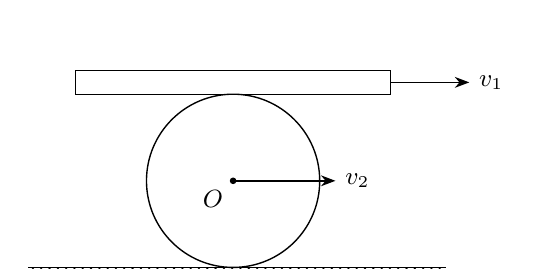
\begin{tikzpicture}[x=1cm,y=1cm,line width=0.5pt,>=Stealth,font=\small]
\draw[fill=white] (0.3,2.2) rectangle (4.3,2.5); \draw[->] (4.3,2.35)--(5.3,2.35) node[right]{$v_1$};
\draw (2.3,1.1) circle(1.1); \fill (2.3,1.1) circle(1.2pt); \node[below left] at (2.3,1.1) {$O$}; \draw[->] (2.3,1.1)--(3.6,1.1) node[right]{$v_2$};
\draw (-0.3,0)--(5.0,0); \fill[pattern=north east lines,draw=none] (-0.3,-0.15) rectangle (5.0,0);
\end{tikzpicture}\par\smallskip
\opt{A}{5}
\opt{B}{2,5}
\opt{C}{10}
\opt{D}{7,5}
\end{minipage}\vspace{9pt}\par
\noindent\begin{minipage}{\linewidth}
\textbf{7.}\ Koordinata boşidan 5 m/s tezlikda yölga çiqqan jism 6 s harakatlanib neçançi koordinataga (m) boradi?\par\smallskip
\opt{A}{30}
\opt{B}{15}
\opt{C}{10}
\opt{D}{20}
\end{minipage}\vspace{9pt}\par
\noindent\begin{minipage}{\linewidth}
\textbf{8.}\ $m$ massali, $l$ uzunlikdagi sterjen tik holda suvda suzib yuribdi, uning suvning içidagi qismi 0,8$l$. Sterjenni tik holda suvdan çiqariş uçun zarur bölgan minimal energiya hisoblansin.\par\smallskip
\opt{A}{$0{,}4mgl$}
\opt{B}{$0{,}8mgl$}
\opt{C}{$0{,}35mgl$}
\opt{D}{$0{,}25mgl$}
\end{minipage}\vspace{9pt}\par
\noindent\begin{minipage}{\linewidth}
\textbf{9.}\ Quyidagi grafikda jism tezligining köçişiga boğliqlik grafigi keltirilgan. Jismning tezlanişini (m/s$^{2}$) aniqlang.\par\smallskip
\noindent\hspace*{4mm}\begin{tikzpicture}[x=1cm,y=1cm,line width=0.5pt,>=Stealth,font=\small]
\draw[->] (0,0)--(4.6,0) node[right]{$S,\mathrm{m}$}; \draw[->] (0,0)--(0,3.0) node[above]{$\vartheta,\mathrm{m/s}$};
\draw[very thick] (0.8,1.5) .. controls (1.2,2.4) and (2.0,2.6) .. (3.6,2.6) ;
\draw[dashed] (0,1.5)--(0.8,1.5)--(0.8,0) (0,2.6)--(3.6,2.6)--(3.6,0);
\node[left] at (0,1.5) {$4$}; \node[left] at (0,2.6) {$6$}; \node[below] at (0.8,0) {$2$}; \node[below] at (3.6,0) {$4{,}5$};
\end{tikzpicture}\par\smallskip
\opt{A}{40}
\opt{B}{2}
\opt{C}{100}
\opt{D}{4}
\end{minipage}\vspace{9pt}\par
\noindent\begin{minipage}{\linewidth}
\textbf{10.}\ Quyida ifodalangan qonunni qanday nomlasa böladi? Agar jism bir neça kuç ta’sirida harakatlanayotgan bölsa, har bir kuç boşqa kuçlar bilan birgalikda yoki yakka ö ta’sir qilayotganidan qat’iy nazar jismga hamma vaqt bir xil tezlaniş beradi.\par\smallskip
\opt{A}{kuçlar ta’sirining mustaqillik qonuni}
\opt{B}{inersiya qonuni}
\opt{C}{impulsning saqlaniş qonuni}
\opt{D}{Nyutonning II qonuni}
\end{minipage}\vspace{9pt}\par
\noindent\begin{minipage}{\linewidth}
\textbf{11.}\ Ideal gazning absolyut temperaturasi 2 marta ortganda uning bosimi 50 \% ga ortdi. Gazning hajmi neça marta özgargan?\par\smallskip
\opt{A}{4/3 marta kamaygan}
\opt{B}{5/3 marta ortgan}
\opt{C}{5/3 marta kamaygan}
\opt{D}{4/3 marta ortgan}
\end{minipage}\vspace{9pt}\par
\noindent\begin{minipage}{\linewidth}
\textbf{12.}\ Hajmlari 100 l va 250 l bölgan ikkita idişda bir xil temperaturali havo bor. Birinçisidagi havoning nisbiy namligi 25 \%. Idişlar birlaştirilgaç havoning nisbiy namligi 35 \% bölib qoldi. Ikkinçi idişdagi havoning nisbiy namligi (\%) dastlab qanday bölgan? (Jarayon izotermik)\par\smallskip
\opt{A}{10}
\opt{B}{39}
\opt{C}{60}
\opt{D}{50}
\end{minipage}\vspace{9pt}\par
\noindent\begin{minipage}{\linewidth}
\textbf{13.}\ 1,204$\cdot10^{24}$ ta molekuladan tarkib topgan gazning modda miqdorini toping (mol). NA =6,02$\cdot10^{23}$ mol$-$1.\par\smallskip
\opt{A}{0,2}
\opt{B}{20}
\opt{C}{2}
\opt{D}{200}
\end{minipage}\vspace{9pt}\par
\noindent\begin{minipage}{\linewidth}
\textbf{14.}\ Yuzasi 1 m$^{2}$ bölgan silindrda 200 N oğirlikdagi erkin siljiy oladigan porşen bor. Agar gaz hajmi 10 l ga kamaysa, taşqi kuçlarning bajargan işini toping (J). Taşqi atmosfera bosimini hisobga olmang.\par\smallskip
\opt{A}{1}
\opt{B}{3}
\opt{C}{2}
\opt{D}{4}
\end{minipage}\vspace{9pt}\par
\noindent\begin{minipage}{\linewidth}
\textbf{15.}\ Massalari örtaça 17,4 $\mu$g dan bölgan çang zarralari havoda uçib yuribdi. Agar havoning molyar massasi 29 g/mol ga teng bölsa, çang zarralari va havo molekulalarining örtaça kvadratik tezliklarini taqqoslang. NA =6$\cdot10^{23}$ mol$-$1.\par\smallskip
\opt{A}{çang zarralari tezligi 600 mln marta katta}
\opt{B}{havo molekulalari tezligi 600 mln marta katta}
\opt{C}{havo molekulalari tezligi 100 mln marta katta}
\opt{D}{bir xil}
\end{minipage}\vspace{9pt}\par
\noindent\begin{minipage}{\linewidth}
\textbf{16.}\ Akkumulyator EYuK 12 V, töplagan zaryadi 60 A$\cdot$h. Uning içki qarşiligi 0,5 $\Omega$, taşqi zanjir qarşiligi 11,5 $\Omega$ bölsa, akkumulyator taşqi zanjirga qança energiya (kJ) bera oladi?\par\smallskip
\opt{A}{2376}
\opt{B}{2484}
\opt{C}{1980}
\opt{D}{2070}
\end{minipage}\vspace{9pt}\par
\noindent\begin{minipage}{\linewidth}
\textbf{17.}\ E.Yu.K $E$, içki qarşiligi $r$ bölgan $n$ ta tok manbai özaro ketma-ket ulandi va batareya hosil qilindi. Agar batareyaga $R$ taşqi qarşilik ulansa, zanjirdagi tok kuçi qanday böladi? $R\gg n\cdot r$.\par\smallskip
\opt{A}{$\approx\dfrac{E}{R}$}
\opt{B}{$\approx\dfrac{E}{nR}$}
\opt{C}{$\approx\dfrac{nE}{R}$}
\opt{D}{$\approx\dfrac{E}{nr}$}
\end{minipage}\vspace{9pt}\par
\noindent\begin{minipage}{\linewidth}
\textbf{18.}\ Qarşiligi 2 $\Omega$ dan bölgan 6 ta ötkazgiç juftlab parallel ulandi. Uçala juft öz navbatida içki qarşiligi 1 $\Omega$ bölgan batareyaga ketma-ket ulandi. Bunda har bir ötkazgiçdan 2,5 A tok ötdi. Agar ulardan biri uzilsa, zanjirdagi tok kuçi qanday böladi (A)?\par\smallskip
\opt{A}{1}
\opt{B}{2}
\opt{C}{4}
\opt{D}{6}
\end{minipage}\vspace{9pt}\par
\noindent\begin{minipage}{\linewidth}
\textbf{19.}\ Ikki musbat zaryadlardan birining miqdori 3 marta orttirilsa, ular orasidagi ta’sir kuçi qanday özgaradi?\par\smallskip
\opt{A}{3 marta ortadi}
\opt{B}{3 marta kamayadi}
\opt{C}{özgarmaydi}
\opt{D}{9 marta ortadi}
\end{minipage}\vspace{9pt}\par
\noindent\begin{minipage}{\linewidth}
\textbf{20.}\ Tebraniş konturi induktivligi 0,5 H bölgan ğaltak va siğimi 20 mF bölgan kondensatordan iborat. Agar kondensatordagi kuçlaniş 2 V bölgan paytda ğaltakdagi tok kuçi 0,3 A bölgan bölsa, konturdagi tok kuçining maksimal qiymatini (A) aniqlang.\par\smallskip
\opt{A}{0,4}
\opt{B}{0,5}
\opt{C}{0,6}
\opt{D}{0,8}
\end{minipage}\vspace{9pt}\par
\noindent\begin{minipage}{\linewidth}
\textbf{21.}\ Qarşiliklari $R_1$ = 6 $\Omega$ va $R_2$ = 12 $\Omega$ bölgan ötkazgiçlar $U$ = 36 V tok manbayiga ketma-ket ulandi. $R_2$ qarşilikdagi kuçlanişni (V) toping.\par\smallskip
\opt{A}{12}
\opt{B}{18}
\opt{C}{24}
\opt{D}{6}
\end{minipage}\vspace{9pt}\par
\noindent\begin{minipage}{\linewidth}
\textbf{22.}\ Özgaruvçan tok manbayiga induktivligi 25 mH bölgan ğaltak ulangan. Agar zanjirdagi tok $i = 4\cos(100\pi t)$ [A] qonun bilan özgarsa, ğaltak uçlaridagi kuçlaniş qanday qonun bilan özgarişini (V) aniqlang.\par\smallskip
\opt{A}{$u = 10\pi\cos(100\pi t + \dfrac{\pi}{2})$}
\opt{B}{$u = 10\pi\cos(100\pi t)$}
\opt{C}{$u = 10\pi\cos(100\pi t - \dfrac{\pi}{2})$}
\opt{D}{$u = -10\pi\cos(100\pi t)$}
\end{minipage}\vspace{9pt}\par
\noindent\begin{minipage}{\linewidth}
\textbf{23.}\ Texnik qöllanmalarda galvanostegiyaning qöllanilişiga doir ma’lumotda h/ kattalik keltiriladi. Bu kattalik nimani ifodalaydi? 1) birlik tok ziçligida qoplaş qalinligining ortiş tezligi; 2) metall elektrokimyoviy ekvivalentini uning ziçligiga nisbati; 3) sarf böladigan energiya miqdori.\par\smallskip
\opt{A}{3}
\opt{B}{2,3}
\opt{C}{1,3}
\opt{D}{1,2}
\end{minipage}\vspace{9pt}\par
\noindent\begin{minipage}{\linewidth}
\textbf{24.}\ Zaryadlangan jism atrofidagi elektr maydon kuç çiziqlari jism sirtiga nisbatan qanday joylaşadi?\par\smallskip
\opt{A}{parallel}
\opt{B}{tik}
\opt{C}{qiya}
\opt{D}{ixtiyoriy}
\end{minipage}\vspace{9pt}\par
\noindent\begin{minipage}{\linewidth}
\textbf{25.}\ E.Yu.K $\varepsilon$ bölgan tok manbai taşqi zanjirga ulanmagan. Mazkur holatda manba qutblaridagi $U$ kuçlanişni toping.\par\smallskip
\opt{A}{$U=\varepsilon$}
\opt{B}{0}
\opt{C}{$U<\varepsilon$}
\opt{D}{$U>\varepsilon$}
\end{minipage}\vspace{9pt}\par
\noindent\begin{minipage}{\linewidth}
\textbf{26.}\ Optik kuçi 6 dptr bölgan yiğuvçi linza yordamida ekranda buyumning 2 marta kiçiklaşgan haqiqiy tasviri hosil qilindi. Buyum va tasvir orasidagi masofani (m) aniqlang\par\smallskip
\opt{A}{1/2}
\opt{B}{3/4}
\opt{C}{2}
\opt{D}{1/4}
\end{minipage}\vspace{9pt}\par
\noindent\begin{minipage}{\linewidth}
\textbf{27.}\ Yiğuvçi linzadan buyumgaça masofa 10 cm ga teng. Linzada buyumning 2 marta kattalaşgan mavhum tasviri hosil bölgan bölsa, uning fokus masofasini (cm) aniqlang.\par\smallskip
\opt{A}{5}
\opt{B}{20}
\opt{C}{50}
\opt{D}{100}
\end{minipage}\vspace{9pt}\par
\noindent\begin{minipage}{\linewidth}
\textbf{28.}\ Fokus masofasi 15 cm bölgan linzada buyumning 3 marta kiçiklaşgan teskari tasviri hosil böldi. Buyumdan tasvirgaça bölgan masofani (cm) aniqlang.\par\smallskip
\opt{A}{80}
\opt{B}{60}
\opt{C}{45}
\opt{D}{90}
\end{minipage}\vspace{9pt}\par
\noindent\begin{minipage}{\linewidth}
\textbf{29.}\ Metall sirtiga tuşayotgan fotonning töliq energiyasi 3 eV ga, sirtdan ajralayotgan fotoelektronlarning maksimal kinetik energiyasi esa 2 eV ga teng. Agar fotonning çastotasi 3 marta orttirilsa, fotoelektronlarning maksimal kinetik energiyasi neça marta ortadi?\par\smallskip
\opt{A}{10}
\opt{B}{2}
\opt{C}{4}
\opt{D}{20}
\end{minipage}\vspace{9pt}\par
\noindent\begin{minipage}{\linewidth}
\textbf{30.}\ Proton elektr maydonida 6,4$\cdot10^{11}$ m/s$^{2}$ tezlaniş bilan harakatlanişi uçun elektr maydon kuçlanganligi qanday (kV/m) bölişi kerak?\par\smallskip
\opt{A}{6,64}
\opt{B}{3,32}
\opt{C}{13,28}
\opt{D}{11,72}
\end{minipage}\vspace{9pt}\par
\noindent\begin{minipage}{\linewidth}
\textbf{31.}\ Yoruğlik tezligiga yaqin tezlikda harakatlanayotgan zarraçaning impulsini tinçlikdagi energiyasiga nisbati $P/E_0=1{,}5/c$ ga teng. Zarraça töliq energiyasini uning tinçlikdagi energiyasiga nisbati $E_T/E_0$ ni toping. $c$ - yoruglikning böşliqdagi tezligi.\par\smallskip
\opt{A}{$\approx1{,}8$}
\opt{B}{$\approx2$}
\opt{C}{$\approx2{,}1$}
\opt{D}{$\approx1{,}2$}
\end{minipage}\vspace{9pt}\par
\noindent\begin{minipage}{\linewidth}
\textbf{32.}\ 32 kg massali jism 400 N kuç bilan tik yuqoriga kötarilmoqda. Jism 42 m balandlikka kötarilganda kuçning bajargan işi (J) nimaga teng?\par\smallskip
\opt{A}{16800}
\opt{B}{13440}
\opt{C}{14400}
\opt{D}{18200}
\end{minipage}\vspace{9pt}\par
\newpage\noindent\textbf{33–35-test topşiriqlariga mos keluvçi javoblarni (A–F) javob variantlaridan tanlang.}\par\smallskip
Vakuumda bir-biridan 6 cm masofada turgan $q=+4$ nC va $-q$ zaryadlar orasidagi kesmaning örtasida $A$ nuqta joylaşgan (rasm). $k=9\cdot10^9\ \mathrm{N\cdot m^2/C^2}$.\par\medskip
\begin{center}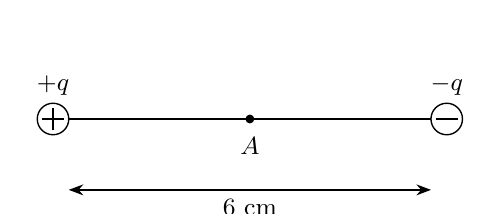
\begin{tikzpicture}[x=1cm,y=1cm,line width=0.5pt,>=Stealth,font=\small]
\draw (0,0)--(5.0,0); \foreach \x/\n in {0/{+q},5.0/{-q}}{\draw[fill=white] (\x,0) circle(0.2); \node[above=5pt] at (\x,0) {$\n$};}
\draw (-0.14,0)--(0.14,0) (0,-0.14)--(0,0.14); \draw (4.86,0)--(5.14,0);
\fill (2.5,0) circle(1.6pt) node[below=3pt]{$A$}; \draw[<->] (0.2,-0.9)--(4.8,-0.9); \node[below] at (2.5,-0.9) {$6\ \mathrm{cm}$};
\end{tikzpicture}\end{center}
\noindent\fbox{\begin{minipage}{0.64\linewidth}\vspace{4pt}\textbf{33.}\ $A$ nuqtadagi elektr maydon kuçlanganligini (kV/m) toping.\\[6pt]\textbf{34.}\ $A$ nuqtadagi maydon potensialini (V) toping.\\[6pt]\textbf{35.}\ $A$ nuqtaga qöyilgan $2$ nC zaryadga ta’sir qiluvçi kuçni ($\mu$N) toping.\vspace{4pt}\end{minipage}\vrule\hspace{6pt}\begin{minipage}{0.28\linewidth}\vspace{4pt}A)\ 0\\B)\ 20\\C)\ 40\\D)\ 80\\E)\ 160\\F)\ 320\vspace{4pt}\end{minipage}}\par\vspace{14pt}
\Needspace{9\baselineskip}
\noindent\textbf{36.}\ Massasi 2 kg bölgan brusok qiyalik burçagi $37^\circ$ bölgan silliq qiya tekislikda bikrligi 200 N/m bölgan prujina yordamida muvozanatda uşlab turilibdi (prujina qiya tekislikka parallel). $\sin37^\circ=0{,}6$, $g=10$ m/s$^2$.\par\smallskip
\medskip\noindent\textbf{a)\ Prujinaning çözilişini (cm) toping.}\par
\noindent\textit{Javob}: a)\ \blank\par
\medskip\noindent\textbf{b)\ Qiya tekislikning brusokka ta’sir qiluvçi normal reaksiya kuçini (N) toping.}\par
\noindent\textit{Javob}: b)\ \blank\par
\medskip\noindent\textbf{Diqqat!} Javoblaringizni javoblar varaqasiga köçirib yozing.\par\vspace{10pt}
\Needspace{9\baselineskip}
\noindent\textbf{37.}\ 20 m balandlikdan gorizontal otilgan jism Yerga gorizontga $45^\circ$ burçak ostida urildi. Havoning qarşiligi hisobga olinmasin, $g=10$ m/s$^2$.\par\smallskip
\medskip\noindent\textbf{a)\ Jismning boşlanğiç tezligini (m/s) toping.}\par
\noindent\textit{Javob}: a)\ \blank\par
\medskip\noindent\textbf{b)\ Jismning gorizontal uçiş uzoqligini (m) toping.}\par
\noindent\textit{Javob}: b)\ \blank\par
\medskip\noindent\textbf{Diqqat!} Javoblaringizni javoblar varaqasiga köçirib yozing.\par\vspace{10pt}
\Needspace{9\baselineskip}
\noindent\textbf{38.}\ Şarça silliq novdan sirpanib tuşib, radiusi 0,4 m bölgan vertikal halqa («ölik sirtmoq») böylab harakatlanadi. Şarçaning massasi 0,1 kg, $g=10$ m/s$^2$.\par\smallskip
\medskip\noindent\textbf{a)\ Şarça halqani uzilmasdan aylanib çiqişi uçun qöyib yuboriladigan eng kiçik balandlikni (m) toping.}\par
\noindent\textit{Javob}: a)\ \blank\par
\medskip\noindent\textbf{b)\ Şarça şu balandlikdan qöyib yuborilganda halqaning eng pastki nuqtasida novga beradigan bosim kuçini (N) toping.}\par
\noindent\textit{Javob}: b)\ \blank\par
\medskip\noindent\textbf{Diqqat!} Javoblaringizni javoblar varaqasiga köçirib yozing.\par\vspace{10pt}
\Needspace{9\baselineskip}
\noindent\textbf{39.}\ Hajmi 2 L bölgan idişda 300 kPa bosimli, hajmi 4 L bölgan idişda 150 kPa bosimli bir xil gaz bor. Idişlar ingiçka nay bilan tutaştirildi, temperatura özgarmaydi.\par\smallskip
\medskip\noindent\textbf{a)\ Idişlardagi qaror topgan bosimni (kPa) toping.}\par
\noindent\textit{Javob}: a)\ \blank\par
\medskip\noindent\textbf{b)\ Birinçi idişdagi bosim neça marta kamaydi?}\par
\noindent\textit{Javob}: b)\ \blank\par
\medskip\noindent\textbf{Diqqat!} Javoblaringizni javoblar varaqasiga köçirib yozing.\par\vspace{10pt}
\Needspace{9\baselineskip}
\noindent\textbf{40.}\ 100 $^\circ$C gaça qizdirilgan 0,5 kg metall jism 20 $^\circ$C temperaturali 0,5 kg suvga tuşirildi. Qaror topgan temperatura 25 $^\circ$C. $c_{suv}=4200$ J/(kg$\cdot$K), issiqlik isroflari yöq.\par\smallskip
\medskip\noindent\textbf{a)\ Suv olgan issiqlik miqdorini (kJ) toping.}\par
\noindent\textit{Javob}: a)\ \blank\par
\medskip\noindent\textbf{b)\ Metallning soliştirma issiqlik siğimini (J/(kg$\cdot$K)) toping.}\par
\noindent\textit{Javob}: b)\ \blank\par
\medskip\noindent\textbf{Diqqat!} Javoblaringizni javoblar varaqasiga köçirib yozing.\par\vspace{10pt}
\Needspace{9\baselineskip}
\noindent\textbf{41.}\ Ideal transformatorning birlamçi çulğamida 1000 öram bölib, u 220 V kuçlanişli tarmoqqa ulangan. Ikkilamçi çulğamda 50 öram bor va unga 5,5 $\Omega$ qarşilikli iste’molçi ulangan.\par\smallskip
\medskip\noindent\textbf{a)\ Ikkilamçi çulğamdagi kuçlanişni (V) toping.}\par
\noindent\textit{Javob}: a)\ \blank\par
\medskip\noindent\textbf{b)\ Birlamçi çulğamdagi tok kuçini (A) toping.}\par
\noindent\textit{Javob}: b)\ \blank\par
\medskip\noindent\textbf{Diqqat!} Javoblaringizni javoblar varaqasiga köçirib yozing.\par\vspace{10pt}
\Needspace{9\baselineskip}
\noindent\textbf{42.}\ Kuçlanganligi 2 kV/m bölgan bir jinsli elektr maydonda $A$ va $B$ nuqtalar bitta kuç çiziğida, bir-biridan 5 cm masofada yotadi; $B$ nuqta $A$ dan maydon yönalişi böylab joylaşgan.\par\smallskip
\medskip\noindent\textbf{a)\ $A$ va $B$ nuqtalar orasidagi potensiallar farqini (V) toping.}\par
\noindent\textit{Javob}: a)\ \blank\par
\medskip\noindent\textbf{b)\ $3\ \mu$C zaryadni $A$ dan $B$ ga köçirişda maydon bajargan işni (mJ) toping.}\par
\noindent\textit{Javob}: b)\ \blank\par
\medskip\noindent\textbf{Diqqat!} Javoblaringizni javoblar varaqasiga köçirib yozing.\par\vspace{10pt}
\Needspace{9\baselineskip}
\noindent\textbf{43.}\ Yoruğlik qalinligi 6 cm bölgan şişa plastinkaga tik tuşmoqda. Şişaning sindiriş körsatkiçi 1,5, $c=3\cdot10^8$ m/s.\par\smallskip
\medskip\noindent\textbf{a)\ Yoruğlikning plastinkadan ötiş vaqtini (ns) toping.}\par
\noindent\textit{Javob}: a)\ \blank\par
\medskip\noindent\textbf{b)\ Plastinkadagi optik yöl uzunligini (cm) toping.}\par
\noindent\textit{Javob}: b)\ \blank\par
\medskip\noindent\textbf{Diqqat!} Javoblaringizni javoblar varaqasiga köçirib yozing.\par\vspace{10pt}
\Needspace{9\baselineskip}
\noindent\textbf{44.}\ Buyum va ekran orasidagi masofa 90 cm. Ular orasiga yiğuvçi linza qöyilganda ekranda buyumning 2 marta kattalaşgan aniq tasviri hosil böldi.\par\smallskip
\medskip\noindent\textbf{a)\ Linzaning fokus masofasini (cm) toping.}\par
\noindent\textit{Javob}: a)\ \blank\par
\medskip\noindent\textbf{b)\ Buyumdan linzagaça masofani (cm) toping.}\par
\noindent\textit{Javob}: b)\ \blank\par
\medskip\noindent\textbf{Diqqat!} Javoblaringizni javoblar varaqasiga köçirib yozing.\par\vspace{10pt}
\Needspace{9\baselineskip}
\noindent\textbf{45.}\ Vodorod atomi asosiy holatining energiyasi $-13{,}6$ eV, birinçi Bor orbitasi radiusi $0{,}53\cdot10^{-10}$ m.\par\smallskip
\medskip\noindent\textbf{a)\ Ikkinçi orbita radiusini ($10^{-10}$ m) toping.}\par
\noindent\textit{Javob}: a)\ \blank\par
\medskip\noindent\textbf{b)\ Ikkinçi energetik sathdagi atomni ionlaştiriş uçun kerak bölgan energiyani (eV) toping.}\par
\noindent\textit{Javob}: b)\ \blank\par
\medskip\noindent\textbf{Diqqat!} Javoblaringizni javoblar varaqasiga köçirib yozing.\par\vspace{10pt}
\end{document}